\documentclass[tikz,border=10pt]{standalone}
\usepackage{tikz}
\usepackage{amsmath}
\usepackage{tikz-3dplot}
\usetikzlibrary{decorations.pathreplacing, decorations.markings, arrows.meta, calc, patterns}

\begin{document}

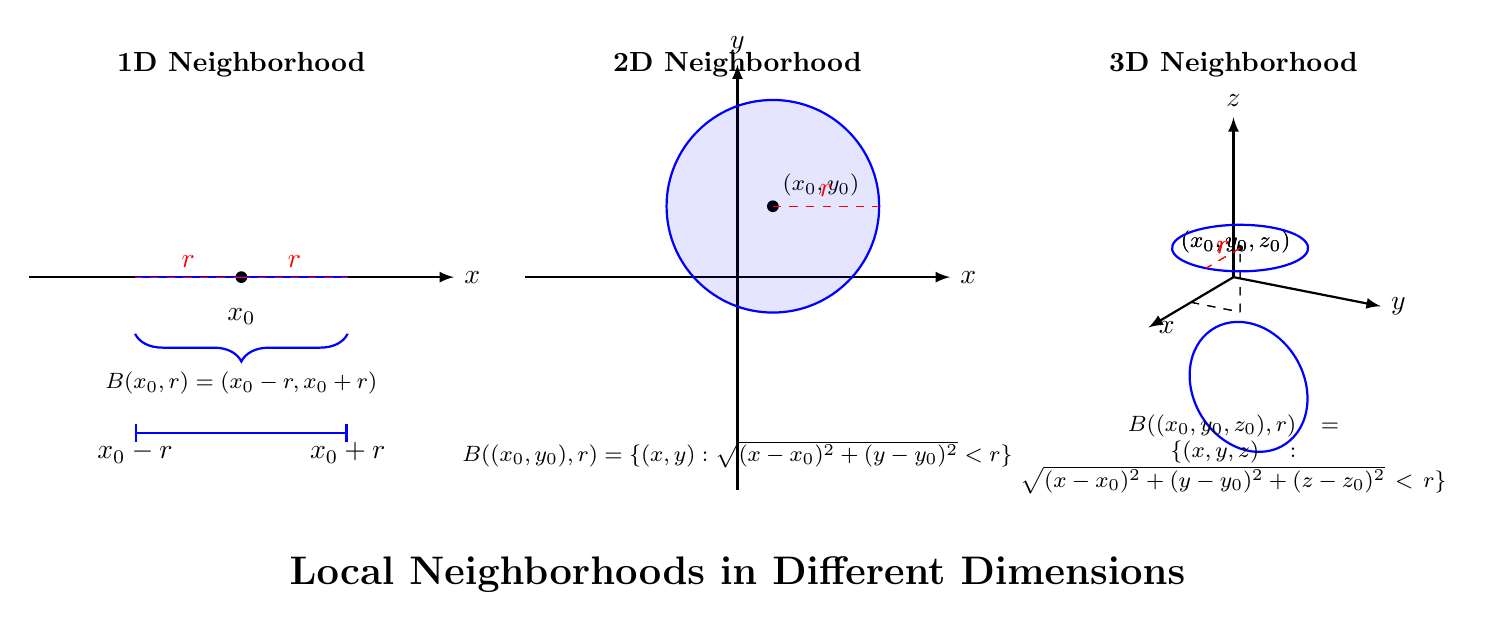
\begin{tikzpicture}[scale=0.9]
% Common styling
\tikzset{
  point/.style={circle, fill, inner sep=1.5pt},
  axes/.style={->, >=latex, thick},
  neighborhood label/.style={font=\footnotesize}
}

% 1D CASE - LEFT
\begin{scope}[xshift=-5cm]
  % Title
  \node at (0, 3) {\textbf{1D Neighborhood}};
  
  % Line (X-axis)
  \draw[axes] (-3,0) -- (3,0) node[right] {$x$};
  
  % Point x_0
  \node[point] (x0) at (0,0) {};
  \node[below] at (0,-0.3) {$x_0$};
  
  % Neighborhood B(x_0, r)
  \draw[thick, blue] (-1.5,0) -- (1.5,0);
  
  % Radius markers
  \draw[dashed, red] (0,0) -- (-1.5,0);
  \draw[dashed, red] (0,0) -- (1.5,0);
  \node[red, above] at (-0.75,0) {$r$};
  \node[red, above] at (0.75,0) {$r$};
  
  % Curly brace decoration below
  \draw[decorate, decoration={brace, mirror, amplitude=10pt}, blue, thick] 
    (-1.5,-0.8) -- (1.5,-0.8);
  
  % Neighborhood label
  \node[neighborhood label] at (0,-1.5) {$B(x_0,r) = (x_0-r, x_0+r)$};
  
  % Interval notation
  \draw[|-|, thick, blue] (-1.5,-2.2) -- (1.5,-2.2);
  \node[below] at (-1.5,-2.2) {$x_0-r$};
  \node[below] at (1.5,-2.2) {$x_0+r$};
\end{scope}

% 2D CASE - MIDDLE
\begin{scope}[xshift=2cm]
  % Title
  \node at (0, 3) {\textbf{2D Neighborhood}};
  
  % Axes
  \draw[axes] (-3,0) -- (3,0) node[right] {$x$};
  \draw[axes] (0,-3) -- (0,3) node[above] {$y$};
  
  % Point (x_0, y_0)
  \node[point] (x0y0) at (0.5,1) {};
  \node[above right, font=\footnotesize] at (0.5,1) {$(x_0,y_0)$};
  
  % Neighborhood B((x_0,y_0), r)
  \draw[thick, blue, fill=blue, fill opacity=0.1] (0.5,1) circle (1.5);
  
  % Radius indicator
  \draw[dashed, red] (0.5,1) -- (2,1);
  \node[red, above] at (1.25,1) {$r$};
  
  % Neighborhood label
  \node[neighborhood label] at (0,-2.5) {$B((x_0,y_0),r) = \{(x,y) : \sqrt{(x-x_0)^2+(y-y_0)^2} < r\}$};
\end{scope}

% 3D CASE - RIGHT
\begin{scope}[xshift=9cm]
  % Title
  \node at (0, 3) {\textbf{3D Neighborhood}};
  
  % 3D Setup
  \tdplotsetmaincoords{70}{120}
  \begin{scope}[tdplot_main_coords, scale=0.8]
    % Axes
    \draw[axes] (0,0,0) -- (3,0,0) node[right] {$x$};
    \draw[axes] (0,0,0) -- (0,3,0) node[right] {$y$};
    \draw[axes] (0,0,0) -- (0,0,3) node[above] {$z$};
    
    % Point (x_0, y_0, z_0)
    \coordinate (x0y0z0) at (1.5,1,1.2);
    \fill[point] (x0y0z0) circle (1.5pt);
    \draw[dashed] (1.5,1,0) -- (x0y0z0);
    \draw[dashed] (1.5,0,0) -- (1.5,1,0);
    \draw[dashed] (0,0,0) -- (1.5,0,0);
    
    % Label for the point
    \node[font=\footnotesize] at (2,1.2,1.5) {$(x_0,y_0,z_0)$};
    
    % Sphere (wireframe only - just two circles)
    % Point (x_0, y_0, z_0)
    \coordinate (x0y0z0) at (1.5,1,1.2);
    \fill[point] (x0y0z0) circle (1.5pt);
    \draw[dashed] (1.5,1,0) -- (x0y0z0);
    \draw[dashed] (1.5,0,0) -- (1.5,1,0);
    \draw[dashed] (0,0,0) -- (1.5,0,0);
    
    % Label for the point
    \node[font=\footnotesize] at (2,1.2,1.5) {$(x_0,y_0,z_0)$};
    
    % Horizontal circle (in the x-y plane at z=1.2)
    \draw[blue, thick] (1.5,1,1.2) circle (1.2);
    
    % Vertical circle (in the x-z plane at y=1)
    \tdplotsetrotatedcoords{0}{90}{0}
    \begin{scope}[tdplot_rotated_coords]
        \draw[blue, thick] (1.5,1,1.2) circle (1.2);
    \end{scope}
    
    % Radius indicator - points to intersection of circles
    \draw[dashed, red] (x0y0z0) -- (2.7,1,1.2);
    \node[red] at (2.1,1,1.4) {$r$};
    
    % Radius indicator
    \draw[dashed, red] (x0y0z0) -- (2.7,1,1.2);
    \node[red] at (2.1,1,1.4) {$r$};
  \end{scope}
  
  % Neighborhood label
  \node[neighborhood label, align=center, text width=6cm] at (0,-2.5) {$B((x_0,y_0,z_0),r) = $ \\ $\{(x,y,z) : \sqrt{(x-x_0)^2+(y-y_0)^2+(z-z_0)^2} < r\}$};
\end{scope}

% Global title
\node at (2,-4.2) {\Large \textbf{Local Neighborhoods in Different Dimensions}};

\end{tikzpicture}

\end{document}
